\chapter{Higher-Order Properties of Bayesian Empirical Likelihood: Univariate
Case}
\section{Introduction}

Empirical likelihood, over the years, has become a very popular topic
of statistical research. The name was coined by Owen in his classic
1986 paper, although similar ideas are found even earlier in the works
of \cite{hartley1968new}%
, \cite{thomas1975confidence}%
, \cite{rubin1981bayesian} and others. The main advantage of empirical
likelihood is that it involves fewer assumptions than a regular likelihood,
and yet shares the same asymptotic properties of the latter. 

Research in this area has primarily been frequentist with a long list
of important theoretical developments accompanied by a large number
of applications. To our knowledge, the first Bayesian work in this
general area appeared in the article of \cite{lazar2003bayesian}
{} followed by some related work in \cite{schennach2005bayesian,schennach2007point}
, the latter introducing the concept of ``exponentially tilted empirical
likelihood''. \cite{lazar2003bayesian} suggested using empirical
likelihood as a substitute for the usual likelihood and carrying out
Bayesian analysis in the usual way. 

Baggerly (1998) \cite{baggerly1998empirical} viewed empirical likelihood as a method
of assigning probabilities to a $n$-cell contingency table in order
to minimize a goodness-of-fit criterion. He selected Cressie--Read
power divergence statistics as one such criterion for construction
of confidence regions in a number of situations and pointed out also
how the usual empirical likelihood, exponentially tilted empirical
likelihood and others could be viewed as special cases of the Cressie--Read
criterion by appropriate choice of the the power parameter. This was
also discussed in \cite{owen2010empirical} who pointed out that
all members of the Cressie--Read family led to ``empirical divergence
analogues of the empirical likelihood in which asymptotic $\chi^{2}$
calibration held for the mean''.

The objective of this article is to provide an asymptotic expansion
of the posterior distribution based on empirical likelihood and its
variations under certain regularity conditions and a mean constraint.
The work is inspired by the work of \cite{fang2006empirical}%
{} who provided a somewhat different expansion subject to a mean constraint.
Unlike \cite{fang2005expected,fang2006empirical}, our result is
based on the derivatives of the pseudo likelihood with respect to
the parameter of interest evaluated at the maximum empirical likelihood estimator,
and a rigorous expansion is provided with particular attention  to the remainder terms. Moreover, we consider a general estimating
equation which includes the mean example of \cite{fang2006empirical}
as a special case. The need for different pseudo-likelihoods for statistical
inference is felt all the more in these days, especially for the analysis
of high-dimensional data, where the usual likelihood based analysis
is hard to perform, These alternative likelihoods are equally valuable
for approximate Bayesian computations , a topic which has only recently
surfaced in the statistics literature (see e.g. \cite{cornuet2008inferring} )%

Asymptotic expansion of the posterior based on a regular likelihood
was given earlier in \cite{johnson1970asymptotic}, and later in
\cite{ghosh1982expansions}. We follow their approach with many necessary
modifications in view of the fact that any meaningful prior needs
to have support in   a data-driven compact set which grows with number of observations. As a special
case of our result, we get the celebrated Bernstein--von Mises theorem.
The latter was mentioned in \cite{lazar2003bayesian} %
for the special case of empirical likelihood, but here we provide
a rigorous  derivation with the needed regularity conditions in a general framework. The asymptotic expansion can also be used in providing asymptotic expansions of the posterior moments, quantiles and other quantities of interest. Moreover, we utilize this asymptotic expansion to find some moment matching priors, earlier given in \cite{ghosh2011moment} based on the regular likelihood.
In constrast to \cite{ghosh2011moment}, the moment matching prior does not depend on the expectation of the derivatives of the log-likelihood function, but depends instead on the second and third central moments of the unbiased estimating function, say $g\left(X,\theta\right)$ . In the particular case, $g\left(X,\theta\right)=X-\theta$ , the prior depends only on knowledge about the second and third central moments of the distribution, and does not require specification of a full likelihood. The moment matching priors differ also  from the reference priors as  introduced in \cite{clarke2010reference}. The latter is an analogue of Jeffreys' prior under most circumstances, with the Godambe information matrix \citep{godambe1960optimum} replacing the Fisher information matrix.


\section{Basic Settings }

Suppose $X_{1},\ldots,X_{n}$ are independent and identically distributed
random  vectors satisfying $E\left\{ g\left(X_{1},\theta\right)\right\} =0$,
where $\theta\in\mathbb{R}$. In this context, \cite{owen1988empirical},
formulated empirical likelihood as a nonparametric likelihood of the
form $\prod_{i=1}^{n}w_{i}\left(\theta\right)$, where $w_{i}$ is
the probability mass assigned to $X_{i}\left(i=1,\ldots,n\right)$
satisfying the constraints 
\begin{equation}
\begin{cases}
w_{i}>0,\mathrm{for\: all\: i;}\\
\sum_{i=1}^{n}w_{i}=1;\\
\sum_{i=1}^{n}w_{i}g\left(X_{i},\theta\right)=0.
\end{cases}\label{eq:constraint-el}
\end{equation}
The target is to maximize $\prod_{i=1}^{n}w_{i}$ or equivalently
$\sum_{i=1}^{n}\log w_{i}$ with respect to $w_{1},\ldots,w_{n}$
subject to the constraints given in Eq. (\ref{eq:constraint-el}). Applying
the Lagrange multiplier method, the solution turns out to be 
\begin{equation}
\hat{w}_{i}^{\mathrm{EL}}\left(\theta\right)=\frac{1}{n\left\{ 1+\nu g\left(X_{i},\theta\right)\right\} },\: i=1,\ldots,n,\label{eq:sol-emp-lik}
\end{equation}
where $\nu$, the Lagrange multiplier satisfies 
\begin{equation}
\sum_{i=1}^{n}\frac{g\left(X_{i},\theta\right)}{1+\nu g\left(X_{i},\theta\right)}=0.\label{eq:lambda-eq}
\end{equation}


It may be noted that in  \cite{fang2005expected,fang2006empirical}%
{}, $g\left(X_{i},\theta\right)=X_{i}-\theta,\:i=1,\ldots,n$. 

Closely related to the empirical likelihood is the exponentially tilted
empirical likelihood where the objective is to maximize the Shannon
entropy $-\sum_{i=1}^{n}w_{i}\log w_{i}$ with the same constraints
in Eq. (\ref{eq:constraint-el}). The resulting solution is 
\[
\hat{w}_{i}^{\mathrm{ET}}\left(\theta\right)=\frac{\exp\left\{ -\nu g\left(X_{i},\theta\right)\right\} }{\sum_{j=1}^{n}\exp\left\{ -\nu g\left(X_{i},\theta\right)\right\} },
\]
where $\nu$, the Lagrange multiplier, satisfies 
\begin{equation}
\sum_{i=1}^{n}\exp\left\{ -\nu g\left(X_{i},\theta\right)\right\} g\left(X_{i},\theta\right)=0.\label{eq:lag-mul-exp-tilt-el}
\end{equation}
The exponentially tilted empirical likelihood is related to Kullback-Leibler
divergence between two empirical distributions, one with weights $w_{i}$
assigned to the $n$ sample points, and the other with uniform weights
$1/n$ assigned to the sample points. 

The general Cressie--Read divergence criterion given by 
\[
\mathrm{CR}\left(\lambda\right)=\frac{2}{\lambda\left(\lambda+1\right)}\sum_{i=1}^{n}\left\{ \left(nw_{i}\right)^{-\lambda}-1\right\} .
\]
We focus on the cases $\lambda\ge0$ and $\lambda\le-1$, because
in these cases, $\mathrm{CR}\left(\lambda\right)$ is a convex function
of the $w_{i}\left(i=1,\ldots,n\right)$, and hence the minimization problem will produce a unique solution.  The limiting cases $\lambda\rightarrow0$
and $\lambda\rightarrow-1$ correspond to the usual empirical likelihood
and the exponentially tilted empirical likelihood as defined earlier. 

For convex $\mathrm{CR}\left(\lambda\right)$, its minimum will be
attained in the compact set $H_{n}$ determined by data. The Lagrange
multiplication method now gives the weights 
\begin{equation}
\hat{w}_{i}^{\mathrm{CR}}\left(\theta\right)=\frac{1}{n}\left\{ \mu+\nu g\left(X_{i},\theta\right)\right\} ^{-1/(\lambda+1)},\, i=1,\ldots,n,\label{eq:weight-cr-el}
\end{equation}
where we abbreviate $\mu\left(\theta\right)$ as $\mu$ and $\nu\left(\theta\right)$ as $\nu$, which
satisfy 
\begin{equation}
\begin{cases}
\sum_{i=1}^{n}\left\{ \mu+\nu g\left(X_{i},\theta\right)\right\} ^{-1/(\lambda+1)}=n,\\
\sum_{i=1}^{n}\left\{ \mu+\nu g\left(X_{i},\theta\right)\right\} ^{-1/(\lambda+1)}X_{i}=0.
\end{cases}\label{eq:lag-mul-cr-el}
\end{equation}


We now introduce the posterior based on an empirical likelihood. The  basic idea was first introduced by \cite{lazar2003bayesian} with several numerical examples. The intuition relies on close relationship between the empirical likelihood and the empirical distribution. \cite{owen2010empirical} formulated the two concepts under the same optimization framework, that is, they shared the same objective function, but the former  was solved under parametric constraints, while the latter was not. Considering this similarity, we can use the empirical likelihood as a valid distribution parameterized by some inferential target. Within the Bayesian paradigm, writing
$\hat{w}_{i}\left(\theta\right)$ as generic notation for either $\hat{w}_{i}^{\mathrm{EL}}$,
$\hat{w}_{i}^{\mathrm{ET}}$ or $\hat{w}_{i}^{\mathrm{CR}}$, and a prior with probability density function $\rho\left(\theta\right)$,
with support in $H_{n}$, the profile (pseudo) posterior is  
\begin{equation}
\pi\left(\theta\mid X_{1},\ldots,X_{n}\right)=\frac{\prod_{i=1}^{n}\hat{w}_{i}\left(\theta\right)\rho\left(\theta\right)}{\int_{H_{n}}\prod_{i=1}^{n}\hat{w}_{i}\left(\theta\right)\rho\left(\theta\right)\diff\theta}.\label{eq:poster-el-expression}
\end{equation}


The main objective of this paper is to provide an asymptotic expansion
of $\pi\left(\theta\mid X_{1},\ldots,X_{n}\right)$. This will include
in particular the Bernstein--von Mises theorem. Towards our main result, we
develop a few necessary lemmas in the next section. Some of these lemmas are also of independent interest as they point out some interesting features pertaining to empirical likelihood. 


\section{Lemmas}

We first point out the natural domain of $\theta$ in empirical likelihood settings. In practice, some values of $\theta$ will result in an empty feasible set under constraints Eq. (\ref{eq:constraint-el}). The set of $\theta$ values which guarantees a non-empty feasible set, and thus a solution of the optimization problem, constitutes a natural domain of the empirical likelihood. One may question whether the size of the natural domain is large enough to contain the true value. The following lemma alleviates this worry.
\begin{lemma}
Assume $g(\cdot,\cdot)$ is a continuous function, then the natural domain defined by the constraints Eq. (\ref{eq:constraint-el}) is a compact set and is nondecreasing with respect to the sample size $n$. 
\end{lemma}
\begin{proof}
By
the third constraint of Eq. (\ref{eq:constraint-el}), $\theta$ is a
continuous function of $w_{1},w_{2},\ldots,w_{n}$, but $w_{i}$ are
defined on a simplex which is a compact set due to the first constraint  of Eq. (\ref{eq:constraint-el}). We may recall that a continuous function
maps compact sets to compact sets. Hence, $\theta$ is naturally defined
on a compact set denoted by $H_n$. 

If all the $g(X_i,\theta),i=1,\ldots,n$ are non-positive or all are non-negative, then the constraints Eq. (\ref{eq:constraint-el}) are violated and $H_n=\emptyset$. Hence, we define the domain as
\begin{eqnarray*}
	H_n&=&\left( \left[\bigcap_{i=1}^n\left\{g\left(X_i,\theta\right)\ge 0\right\}\right]\bigcup  \left[\bigcap_{i=1}^n\left\{g\left(X_i,\theta\right)\le 0\right\}\right] \right)^c\\
	&=& \left[\bigcup_{i=1}^n\left\{g\left(X_i,\theta\right)\ge 0\right\}^c\right]\bigcap  \left[\bigcup_{i=1}^n\left\{g\left(X_i,\theta\right)\le 0\right\}^c\right].
\end{eqnarray*}
As $n$ increases, both $\left\{\left[\bigcup_{i=1}^n\left\{g\left(X_i,\theta\right)\ge 0\right\}^c\right]\right\} $ and 
$\left\{\left[\bigcup_{i=1}^n\left\{g\left(X_i,\theta\right)\le 0\right\}^c\right]\right\} $ will increase, and  so will their intersection $H_n$.
\end{proof}

Although, intuitively we expect the empirical likelihood to behave
as the true likelihood, we need some theoretical support to show that
the former enjoys some of the basic properties of the latter. In particular,
we need to verify that $\nu$ and $\mu$ are smooth functions of $\theta$
and the (pseudo) Fisher Information based on the empirical likelihood
is positive. 

We first establish the positiveness of the Fisher information . We
consider the three cases separately to introduce more transparency
and continuity in our approach. 

Our first lemma shows that the Lagrange multipliers $\nu\left(\theta\right)$
and $\mu\left(\theta\right)$ are both smooth functions of $\theta$, under the following mild assumptions,
\begin{assumption}
\label{ass:denom-not-zero} 
For any $\theta$ in natural domain $H_n$, and $n\ge 3$,
\[
	\mathrm{pr}\left\{ g(X_i,\theta)=0, \: i=1,\ldots,n \right\}=0.
\]
\end{assumption}
And 
\begin{assumption}
\label{ass:first-order-smooth-g}
$g(x,\theta)$ is a continuous multivariate function with continuous derivatives in $\theta$.
\end{assumption}

\begin{lemma}
\label{lem:first-order-smooth-lagmul} Under Assumptions \ref{ass:denom-not-zero} and \ref{ass:first-order-smooth-g}, for the empirical likelihood, exponentially
tilted empirical likelihood and Cressie--Read empirical likelihood$\left(\lambda\right)$,
the Lagrange multipliers $\nu\left(\theta\right)$ and $\mu\left(\theta\right)$
are smooth functions of $\theta.$\end{lemma}
\begin{proof}
We first consider the empirical likelihood and observe that, $\nu\left(\theta\right)$
is a implicit function of $\theta$ in view of (\ref{eq:lambda-eq})
. Further 
\[
\frac{\partial}{\partial\nu}\sum_{i=1}^{n}\frac{g\left(X_{i},\theta\right)}{1+\nu g\left(X_{i},\theta\right)}=-\sum_{i=1}^{n}\frac{g^{2}\left(X_{i},\theta\right)}{\left\{ 1+\nu g\left(X_{i},\theta\right)\right\} ^{2}}<0,
\]
so that by the implicit function theorem, $\nu$ is differentiable
in $\theta$. Moreover, differentiating both sides of Eq. (\ref{eq:lambda-eq})
with respect to $\theta$, one gets
\begin{eqnarray*}
0 & = & \sum_{i=1}^{n}\frac{1}{1+\nu g\left(X_{i},\theta\right)}\frac{\diff g\left(X_{i},\theta\right)}{\diff\theta}-\sum_{i=1}^{n}\frac{\nu g\left(X_{i},\theta\right)}{\left\{ 1+\nu g\left(X_{i},\theta\right)\right\} ^{2}}\frac{\diff g\left(X_{i},\theta\right)}{\diff\theta}\\
 &  & -\sum_{i=1}^{n}\frac{g^{2}\left(X_{i},\theta\right)}{\left\{ 1+\nu g\left(X_{i},\theta\right)\right\} ^{2}}\frac{\diff\nu}{\diff\theta},
\end{eqnarray*}
which on simplification leads to 
\begin{equation}
\frac{\diff\nu}{\diff\theta}=-\frac{\sum_{i=1}^{n}\left\{ 1+\nu g\left(X_{i},\theta\right)\right\} ^{-2}\diff g\left(X_{i},\theta\right)/\diff\theta}{\sum_{i=1}^{n}\left\{ 1+\nu g\left(X_{i},\theta\right)\right\} ^{-2}g^{2}\left(X_{i},\theta\right)},\label{eq:decreasing-theta-to-nu}
\end{equation}


Next, for exponentially tilted empirical likelihood, in view of Eq. (\ref{eq:lag-mul-exp-tilt-el})
and the relation 
\begin{eqnarray*}
 &  & \frac{\diff}{\diff\nu}\left[\sum_{i=1}^{n}\exp\left\{ -\nu g\left(X_{i},\theta\right)\right\} g\left(X_{i},\theta\right)\right]\\
 & = & -\sum_{i=1}^{n}\exp\left\{ -\nu g\left(X_{i},\theta\right)\right\} g^{2}\left(X_{i},\theta\right)<0,
\end{eqnarray*}
 once again, the implicit function theorem guarantees the differentiability
of $\nu$ in $\theta$. Further, differentiating both sides of Eq. (\ref{eq:lag-mul-exp-tilt-el})
with respect to $\theta$, one gets 
\begin{equation}
\frac{\diff\nu}{\diff\theta}=\frac{\sum_{i=1}^{n}\exp\left\{ -\nu\left(\theta\right)g\left(X_{i},\theta\right)\right\} \left\{ \diff g\left(X_{i},\theta\right)/\diff\theta\right\} \left\{ 1-\nu g\left(X_{i},\theta\right)\right\} }{\sum_{i=1}^{n}\exp\left\{ -\nu\left(\theta\right)g\left(X_{i},\theta\right)\right\} g^{2}\left(X_{i},\theta\right)}.\label{eq:first-deri-lag-mult-exp-tilted-el}
\end{equation}


A similar conclusion is achieved for $\nu\left(\theta\right)$ and
$\mu\left(\theta\right)$ defined in Eq. (\ref{eq:lag-mul-cr-el}) in
connection with CR$\left(\lambda\right)$. Specifically, defining
\[
\begin{cases}
F_{1}=\sum_{i=1}^{n}\left\{ \mu+\nu g\left(X_{i},\theta\right)\right\} ^{-1/(\lambda+1)}-n,\\
F_{2}=\sum_{i=1}^{n}\left\{ \mu+\nu g\left(X_{i},\theta\right)\right\} ^{-1/(\lambda+1)}g\left(X_{i},\theta\right),
\end{cases}
\]
it follows that,
\[
\frac{\partial\left(F_{1},F_{2}\right)}{\partial\left(\mu,\nu\right)}=-\frac{1}{\lambda+1}\left(\begin{array}{cc}
\sum_{i=1}^{n}q_{i} & \sum_{i=1}^{n}q_{i} g\left(X_{i},\theta\right)\\
\sum_{i=1}^{n}q_{i} g\left(X_{i},\theta\right) & \sum_{i=1}^{n}q_{i} g\left(X_{i},\theta\right)^{2}
\end{array}\right),
\]
 where $q_{i}=\left\{ \mu+\nu g\left(X_{i},\theta\right)\right\} ^{-1/(\lambda+1)-1}$
. Then the determinant of Jacobian is 
\begin{eqnarray*}
\det\frac{\partial\left(F_{1},F_{2}\right)}{\partial\left(\mu,\nu\right)} & = & \left(\frac{1}{\lambda+1}\right)^{2}\left[\sum_{i=1}^{n}q_{i}\sum_{i=1}^{n}q_{i}g\left(X_{i},\theta\right)^{2}-\left\{ \sum_{i=1}^{n}q_{i}g\left(X_{i},\theta\right)\right\} ^{2}\right]\\
 & = & \left(\frac{1}{\lambda+1}\right)^{2}\left(\sum_{i=1}^{n}q_{i}\right)^{2}\left[\sum_{i=1}^{n}\frac{q_{i}}{\sum_{j=1}^{n}q_{j}}g\left(X_{i},\theta\right)^{2}-\left\{ \sum_{i=1}^{n}\frac{q_{i}}{\sum_{j=1}^{n}q_{j}}g\left(X_{i},\theta\right)\right\} \right]^{2}>0.
\end{eqnarray*}
Again, by implicit function theorem, one gets differentiability of
$\mu\left(\theta\right)$ and $\nu\left(\theta\right)$with respect
to $\theta$, and 
\begin{eqnarray}
\left(\begin{array}{c}
\mu'\\
\nu'
\end{array}\right) & = & \left(\frac{\partial\left(F_{1},F_{2}\right)}{\partial\left(\mu,\nu\right)}\right)^{-1}\left(\begin{array}{c}
\partial F_{1}/\partial\theta\\
\partial F_{2}/\partial\theta
\end{array}\right)\nonumber \\
 & = & \left(-\frac{1}{\lambda+1}\right)\left(\lambda+1\right)^{2}\frac{1}{\sum_{i=1}^{n}q_{i}\sum_{i=1}^{n}q_{i}g\left(X_{i},\theta\right)^{2}-\left\{ \sum_{i=1}^{n}q_{i}g\left(X_{i},\theta\right)\right\} ^{2}}\nonumber \\
 &  & \times\left(\begin{array}{cc}
\sum_{i=1}^{n}q_{i}g\left(X_{i},\theta\right)^{2} & -\sum_{i=1}^{n}q_{i}g\left(X_{i},\theta\right)\\
-\sum_{i=1}^{n}q_{i}g\left(X_{i},\theta\right) & \sum_{i=1}^{n}q_{i}
\end{array}\right)\nonumber \\
& & \times \Bigg(\left(\lambda+1\right)^{-1}\sum_{i=1}^{n}q_{i}\nu\frac{\diff g\left(X_{i},\theta\right)}{\diff\theta}, -\left(\lambda+1\right)\sum_{i=1}^{n}q_{i}\nu g\left(X_{i},\theta\right)\frac{\diff g\left(X_{i},\theta\right)}{\diff\theta}\nonumber \\
 &  & 
+\sum_{i=1}^{n}\left\{ \mu+\nu g\left(X_{i},\theta\right)\right\} ^{-1/(\lambda+1)}\frac{\diff g\left(X_{i},\theta\right)}{\diff\theta}
\Bigg)^T .\label{eq:first-der-lag-mul-crel}
\end{eqnarray}

\end{proof}
The next result shows that all the derivatives of the Lagrange multipliers
$\nu\left(\theta\right)$ and $\mu\left(\theta\right)$ are smooth
functions of $\theta\in H_n$. We provide a unified proof for all three
cases where we utilize the previous lemma. with an assumption stronger than Assumption \ref{ass:first-order-smooth-g},
\begin{assumption}
\label{ass:high-order-smooth-g}
$g(x,\theta)$ is a multivariate continuous function and $(K+4)$th-order differentiable in $\theta$.
\end{assumption}

\begin{lemma}
\label{lem:mul-el-smooth-lagrange-mul-1}Under Assumptions \ref{ass:denom-not-zero} and \ref{ass:high-order-smooth-g}, all derivatives of $\nu\left(\theta\right)$
and $\mu\left(\theta\right)$ are smooth functions of $\theta$ for
$\theta\in H_n$.\end{lemma}
\begin{proof}
The result is proved by induction. We have seen already in Lemma \ref{lem:first-order-smooth-lagmul}, that 
the first derivatives of  $\nu'\left(\theta\right)$ and $\mu'\left(\theta\right)$
are smooth functions of $\theta$. Suppose the result holds for all
$k$th derivatives of $\nu\left(\theta\right)$ and $\mu\left(\theta\right)$
for $k=1,\ldots,K$. Then writing 
\[
\frac{\diff^{k}\nu}{\diff\theta^{k}}=h_{k}\left\{ \nu\left(\theta\right),\theta\right\} ,k=1,\ldots,K,
\]
 
\[
\frac{\diff^{k+1}\nu}{\diff^{k+1}\theta}=\frac{\partial h_{k}}{\partial\nu}\frac{\diff\nu}{\diff\theta}+\frac{\partial h_{k}}{\partial\theta}
\]
which is also a smooth function of $\theta$ by the induction hypothesis
and Lemma 1. A similar proof works for $\mu\left(\theta\right)$.
\end{proof}
We know that when the number of constraints and dimension of the parameters
are the same, the corresponding empirical likelihood is maximized
at $\theta=\tilde{\theta}$, the $M$-estimator of $\theta$ based on
$\sum_{i=1}^{n}g\left(X_{i},\theta\right)=0$. Thus, $\nu\left(\tilde{\theta}\right)=0$
and $\mu\left(\tilde{\theta}\right)=1$. We next show that $\tilde{l}\left(\theta\right)$
has a negative second order derivative when evaluated at $\tilde{\theta}$.
\begin{lemma}
\label{lem:bell-shape-el} %
 Under  Assumptions \ref{ass:denom-not-zero} and \ref{ass:first-order-smooth-g},
$\diff^{2}\tilde{l}\left(\tilde{\theta}\right)/\diff\theta^{2}<0$
where $\tilde{l}\left(\theta\right)=n^{-1}\sum_{i=1}^{n}\log\hat{w}_{i}\left(\theta\right)$
where $\hat{w}_{i}$ is either $\hat{w}_{i}^{\mathrm{EL}}$, $\hat{w}_{i}^{\mathrm{ET}}$
or $\hat{w}_{i}^{\mathrm{CR}}$ $\left(i=1,\ldots,n\right)$.\end{lemma}
\begin{proof}
We begin with $\tilde{l}\left(\theta\right)=n^{-1}\sum_{i=1}^{n}\log\hat{w}_{i}^{\mathrm{EL}}\left(\theta\right)=-\sum_{i=1}^{n}\log\left\{ 1+\nu\left(X_{i}-\theta\right)\right\} -\log n$.
Hence by Eq. (\ref{eq:sol-emp-lik}), Eq. (\ref{eq:lambda-eq}) and Eq. (\ref{eq:decreasing-theta-to-nu}),
\begin{eqnarray*}
\frac{\diff\tilde{l}\left(\theta\right)}{\diff\theta}&=&\frac{1}{n}\nu\left(\theta\right)\sum_{i=1}^{n}\frac{1}{1+\nu g\left(X_{i}\theta\right)}\frac{\diff g\left(X_{i},\theta\right)}{\diff\theta}-\frac{1}{n}\sum_{i=1}^{n}\frac{g\left(X_{i}\theta\right)}{1+\nu g\left(X_{i}\theta\right)}\frac{\diff\nu}{\diff\theta}\\
&=&\frac{1}{n}\nu\left(\theta\right)\sum_{i=1}^{n}\frac{1}{1+\nu g\left(X_{i}\theta\right)}\frac{\diff g\left(X_{i},\theta\right)}{\diff\theta}.
\end{eqnarray*}


Thus 
\[
\left.\frac{\diff^{2}\tilde{l}\left(\theta\right)}{\diff\theta^{2}}\right|_{\theta=\tilde{\theta}}=-\frac{\left\{ \sum_{i=1}^{n}\diff g\left(X_{i},\tilde{\theta}\right)/\diff\theta\right\} ^{2}}{n\sum_{i=1}^{n}g^{2}\left(X_{i},\tilde{\theta}\right)}<0.
\]


Next we consider $\tilde{l}\left(\theta\right)=n^{-1}\sum_{i=1}^{n}\log\hat{w}_{i}^{\mathrm{ET}}\left(\theta\right)=-\nu n^{-1}\sum_{i=1}^{n}g\left(X_{i},\theta\right)-\log\sum_{i=1}^{n}\exp\left\{ -\nu g\left(X_{i},\theta\right)\right\} $.
Then 
\begin{eqnarray*}
\frac{\diff\tilde{l}\left(\theta\right)}{\diff\theta} & = & -\frac{\diff\nu}{\diff\theta}\frac{1}{n}\sum_{i=1}^{n}g\left(X_{i},\theta\right)\\
 &  & +\frac{\sum_{i=1}^{n}\exp\left\{ -\nu g\left(X_{i},\theta\right)\right\} \left\{ \left(\diff\nu/\diff\theta\right) g\left(X_{i},\theta\right)+\nu\diff g\left(X_{i},\theta\right)/\diff\theta\right\} }{\sum_{i=1}^{n}\exp\left\{ -\nu g\left(X_{i},\theta\right)\right\} }\\
 & = & -\frac{\diff\nu}{\diff\theta}\frac{1}{n}\sum_{i=1}^{n}g\left(X_{i},\theta\right)+\nu\frac{\sum_{i=1}^{n}\exp\left\{ -\nu g\left(X_{i},\theta\right)\right\} \diff g\left(X_{i},\theta\right)/\diff\theta}{\sum_{i=1}^{n}\exp\left\{ -\nu g\left(X_{i},\theta\right)\right\} }\\
 &  & -\nu n^{-1}\sum_{i=1}^{n}\frac{\diff g\left(X_{i},\theta\right)}{\diff\theta}.
\end{eqnarray*}
Thus, by Eq. (\ref{eq:decreasing-theta-to-nu})
\[
\left.\frac{\diff^{2}\tilde{l}\left(\theta\right)}{\diff\theta^{2}}\right|_{\theta=\tilde{\theta}}=-\frac{\diff\nu}{\diff\theta}\frac{1}{n}\sum_{i=1}^{n}\frac{\diff g\left(X_{i},\tilde{\theta}\right)}{\diff\theta}=-\frac{\left\{ \sum_{i=1}^{n}\diff g\left(X_{i},\tilde{\theta}\right)/\diff\theta\right\} ^{2}}{n\sum_{i=1}^{n}g^{2}\left(X_{i},\tilde{\theta}\right)}<0.
\]


Finally, for the Cressie--Read case, $\tilde{l}\left(\theta\right)=n^{-1}\sum_{i=1}^{n}\log\hat{w}_{i}^{\mathrm{CR}}\left(\theta\right)=-\left\{ n\left(\lambda+1\right)\right\} ^{-1}\sum_{i=1}^{n}\log\left\{ \mu+\nu g\left(X_{i},\theta\right)\right\} $.
Then by Eq. (\ref{eq:first-der-lag-mul-crel}), 
\[
\left.\frac{\diff^{2}\tilde{l}\left(\theta\right)}{\diff\theta^{2}}\right|_{\theta=\tilde{\theta}}=-\frac{\left\{ \sum_{i=1}^{n}\diff g\left(X_{i},\tilde{\theta}\right)/\diff\theta\right\} ^{2}}{n\sum_{i=1}^{n}g^{2}\left(X_{i},\tilde{\theta}\right)}.
\]

\end{proof}
Let $b=\left[\left\{ n^{-1}\sum_{i=1}^{n}\diff g\left(X_{i},\tilde{\theta}\right)/\diff\theta\right\} ^{2}/\left\{ n^{-1}\sum_{i=1}^{n}g\left(X_{i},\tilde{\theta}\right)^{2}\right\} \right]^{-1/2}$.
The main result is proved in the next section.


\section{Main Result}

Before stating the main theorem, we need a few notations. We assume that the
prior density $\rho\left(\theta\right)$ has a $K$th-order continuous derivative
at $\tilde{\theta}$. Let $\rho_{K}\left(\theta\right)=\rho\left(\tilde{\theta}\right)+\rho'\left(\tilde{\theta}\right)\left(\theta-\tilde{\theta}\right)+\cdots+\rho^{\left(K\right)}\left(\tilde{\theta}\right)\left(\theta-\tilde{\theta}\right)$ the $K$th-order  Taylor approximation of the prior density.
Further denote the higher-order derivatives of (pseudo) log empirical
likelihood as 
\[
a_{kn}\left(\theta\right)=\frac{1}{k!}\sum_{i=1}^{n}\frac{\diff^{k}\tilde{l}\left(\theta\right)}{\diff\theta^{k}},\: k=3,\ldots,K+3.
\]
 Define the summation index set 
\[
I_{i,k}=\left\{ \left(m_{3,i},\ldots,m_{K+3,i}\right)\in\mathbb{N}^{K}:\sum_{u=3}^{K+3}m_{u,i}=i,\:\sum_{u=3}^{K+3}m_{u,i}\left(u-2\right)=k\right\} .
\]
 Let $y=\sqrt{n}b\left(\theta-\tilde{\theta}\right)$ be the normalized posterior random variable and 
\begin{eqnarray*}
\alpha_{k}\left(y,n\right) & = & \frac{1}{k!}\rho^{\left(k\right)}\left(\tilde{\theta}\right)\left(\frac{y}{b}\right)^{k}+\sum_{j=0}^{k-1}\frac{1}{j!}\rho^{\left(j\right)}\left(\tilde{\theta}\right)\\
 &  & \times\sum_{i=\left\lceil \left(k-j\right)/\left(K+1\right)\right\rceil }^{k-j}\frac{1}{i!}\sum_{I_{i,k-j}}\binom{i}{m_{3,i},\ldots,m_{K+3,i}}\prod_{u=3}^{K+3}\left\{ a_{un}\left(\tilde{\theta}\right)\right\} ^{m_{u,i}}\left(\frac{y}{b}\right)^{k+2i+j},
\end{eqnarray*}
where, $k=0,\ldots,K$. For special cases $k=0,1$, we have $\alpha_{0}\left(y,n\right)=\rho\left(\tilde{\theta}\right)$
and $\alpha_{1}\left(y,n\right)=\rho'\left(\tilde{\theta}\right)y/b+\rho\left(\tilde{\theta}\right)a_{3n}\left(\tilde{\theta}\right)\left(y/b\right)^{3}.$
Now define $Y_{\left(1\right)}=\sqrt{n}b\left(h_{1}-\tilde{\theta}\right)$
and $Y_{\left(n\right)}=\sqrt{n}b\left(h_{2}-\tilde{\theta}\right)$  as  the normalized lower and upper bounds of the support of the  distribution. Now for any $\xi\in\left(Y_{\left(1\right)},Y_{\left(n\right)}\right)$ 
and $H_n=\left[h_{1},h_{2}\right]$, {let }
\[
P_{K}\left(\xi,n\right)=\sum_{k=0}^{K}\left\{ \int_{Y_{\left(1\right)}}^{\xi}\alpha_{k}\left(y,n\right)\exp\left(-\frac{y^{2}}{2}\right)\diff y\right\} n^{-k/2}.
\]
To control the higher-order error terms, we need the following assumptions.
\begin{assumption}
\label{ass:higher-order-moment-deriv-g}
For any $\left(l_1,\ldots,l_j\right)\subset\left\{2,\ldots,K+3\right\}$,
\[
	E\left\{\prod_{i=1}^j \frac{\diff^{l_i} g\left(X_1,\theta\right)}{\diff \theta^{l_i}}\right\} < \infty.
\]
\end{assumption}
Moreover, we also need an assumption to guarantee the consistency of $M$-Estimator,
\begin{assumption}
\label{ass:m-est-consistency}
$g\left(\cdot,\theta\right)$ is either bounded or monotone in $\theta$.
\end{assumption} 
Now we state the main theorem of this section.
\begin{theorem}[Fundamental Theorem for Expansion]
\label{thm:main-thm}Let $X_{1},X_{2},\ldots,X_{n}$ be independent and identically distributed.   %
Assume the prior density $\rho\left(\theta\right)$ has a support containing
$H_n$ and has $\left(K+1\right)$th-order continuous derivative. Under Assumptions \ref{ass:denom-not-zero} , \ref{ass:high-order-smooth-g} ,\ref{ass:higher-order-moment-deriv-g} and \ref{ass:m-est-consistency},  there
exist constants $N_{1}>0$ and $M_{1}>0$, such that 
\begin{equation}
\left|\int_{Y_{\left(1\right)}}^{\xi}\prod_{i=1}^{n}\hat{w}_{i}\left(\tilde{\theta}+\frac{y}{\sqrt{n}b}\right)\rho\left(\tilde{\theta}+\frac{y}{\sqrt{n}b}\right)\diff y-P_{K}\left(\xi,n\right)\right|\le M_{1}n^{-\left(K+1\right)/2},\ascv\label{eq:fund-exp-formula}
\end{equation}
for any $n>N_{1}$ and $\xi\in\left(Y_{\left(1\right)},Y_{\left(n\right)}\right)$. \end{theorem}
\begin{proof}
See Appendix \ref{app-proof-fun-thm}.
\end{proof}
This theorem can not only be used to prove asymptotic expansion of
the posterior cumulative distribution function , the main result of this
paper, but it can also be used to find the asymptotic expansions of the
posterior mean, quantiles and many other quantities of interest, as in \cite{johnson1970asymptotic}
and \cite{vexler2014posterior} . 

Next we write the posterior cumulative distribution function as 
\[
\Pi\left(\left.\theta\le\tilde{\theta}+\frac{\xi}{\sqrt{n}b}\right|X_{1},\ldots,X_{n}\right)=\frac{\int_{h_{1}}^{\tilde{\theta}+\xi/\sqrt{n}b}\prod_{i=1}^{n}\hat{w}_{i}\left(\theta\right)\rho\left(\theta\right)\diff\theta}{\int_{h_{1}}^{h_{2}}\prod_{i=1}^{n}\hat{w}_{i}\left(\theta\right)\rho\left(\theta\right)\diff\theta}.
\]
Moreover, let $R_{n}=\left(Y_{\left(1\right)},Y_{\left(n\right)}\right)$
and 
\[
\Phi\left(\xi\mid R_{n}\right)=\frac{\int_{Y_{\left(1\right)}}^{\xi}\varphi\left(y\right)\diff y}{\int_{Y_{\left(1\right)}}^{Y_{\left(n\right)}}\varphi\left(y\right)\diff y},
\]
where $\varphi\left(y\right)$ is standard normal density, be restricted
to $R_{n}$. Define polynomial $\gamma_{i}\left(\xi,n\right),\: i=1,\ldots,n$
recursively as 
\[
\int_{Y_{\left(1\right)}}^{\xi}\alpha_{k}\left(y,n\right)\exp\left(-\frac{y^{2}}{2}\right)\diff y=\sum_{j=0}^{k}\left\{ \int_{Y_{\left(1\right)}}^{Y_{\left(n\right)}}\alpha_{j}\left(y,n\right)\exp\left(-\frac{y^{2}}{2}\right)\diff y\right\} \gamma_{k-j}\left(\xi,n\right).
\]
The first two terms of $\gamma_{i}\left(\xi,n\right)$ are
\[
\gamma_{0}\left(\xi,n\right)=\frac{\rho\left(\tilde{\theta}\right)\int_{Y_{\left(1\right)}}^{\xi}\exp\left(-y^{2}/2\right)\diff y}{\rho\left(\tilde{\theta}\right)\int_{Y_{\left(1\right)}}^{Y_{\left(n\right)}}\exp\left(-y^{2}/2\right)\diff y}=\frac{\Phi\left(\xi\right)-\Phi\left(Y_{\left(1\right)}\right)}{\Phi\left(Y_{\left(n\right)}\right)-\Phi\left(Y_{\left(1\right)}\right)}-=\Phi\left(\xi\mid R_{n}\right),
\]
and 
\begin{eqnarray*}
\gamma_{1}\left(\xi,n\right) & = & \frac{\int_{Y_{\left(1\right)}}^{\xi}\exp\left(-y^{2}/2\right)\left\{ \rho'\left(\tilde{\theta}\right)y/b+\rho\left(\tilde{\theta}\right)a_{3n}\left(\tilde{\theta}\right)\left(y/b\right)^{3}\right\} \diff y}{\rho\left(\tilde{\theta}\right)\int_{Y_{\left(1\right)}}^{Y_{\left(n\right)}}\exp\left(-y^{2}/2\right)\diff y}\\
 &  & -\frac{\int_{Y_{\left(1\right)}}^{Y_{\left(n\right)}}\exp\left(-y^{2}/2\right)\left\{ \rho'\left(\tilde{\theta}\right)y/b+\rho\left(\tilde{\theta}\right)a_{3n}\left(\tilde{\theta}\right)\left(y/b\right)^{3}\right\} \diff y}{\rho\left(\tilde{\theta}\right)\int_{Y_{\left(1\right)}}^{Y_{\left(n\right)}}\exp\left(-y^{2}/2\right)\diff y}\Phi\left(\xi\mid R_{n}\right)\\
 & = & \left\{ \frac{\rho'\left(\tilde{\theta}\right)}{b\rho\left(\tilde{\theta}\right)}\right\} \frac{\varphi\left(Y_{\left(1\right)}\right)-\varphi\left(\xi\right)-\Phi\left(\xi\mid R_{n}\right)\left\{ \varphi\left(Y_{\left(1\right)}\right)-\varphi\left(Y_{\left(n\right)}\right)\right\} }{\int_{Y_{\left(1\right)}}^{Y_{\left(n\right)}}\varphi\left(y\right)\diff y}\\
 &  & +\left\{ \frac{a_{3n}\left(\tilde{\theta}\right)}{b^{3}}\right\} \Bigg\{\frac{Y_{\left(1\right)}^{2}\varphi\left(Y_{\left(1\right)}\right)+2\varphi\left(Y_{\left(1\right)}\right)-\xi^{2}\varphi\left(\xi\right)-2\varphi\left(\xi\right)}{\int_{Y_{\left(1\right)}}^{Y_{\left(n\right)}}\varphi\left(y\right)\diff y}\\
 &  & -\Phi\left(\xi\mid R_{n}\right)\frac{Y_{\left(1\right)}^{2}\varphi\left(Y_{\left(1\right)}\right)+2\varphi\left(Y_{\left(1\right)}\right)-Y_{\left(n\right)}^{2}\varphi\left(Y_{\left(n\right)}\right)-2\varphi\left(Y_{\left(n\right)}\right)}{\int_{Y_{\left(1\right)}}^{Y_{\left(n\right)}}\varphi\left(y\right)\diff y}\Bigg\}.
\end{eqnarray*}
 

We now provide the next important result result of this section, namely the asymptotic
expansion of the posterior distribution function.
\begin{theorem}[Asymptotic Expansion of the Posterior Cumulative Distribution Function]
\label{thm:asym-exp-post-cdf} Use the same assumptions as in Theorem
\ref{thm:main-thm}. Then there exist constants $N_{2}$ and $M_{2}$,
such that 
\begin{equation}
\left|\Pi\left(\left.\theta\le\tilde{\theta}+\frac{\xi}{\sqrt{n}b}\right|X_{1},\ldots,X_{n}\right)-\Phi\left(\xi\mid R_{n}\right)-\sum_{i=1}^{K}\gamma_{i}\left(\xi,n\right)n^{-i/2}\right|\le M_{2}n^{-\left(K+1\right)/2},\ascv,\label{eq:asym-exp-post-prob}
\end{equation}
for any $n\ge N_{2}$ and $\xi\in\left(Y_{\left(1\right)},Y_{\left(n\right)}\right)$. \end{theorem}
\begin{proof}
By Theorem \ref{thm:main-thm}, we have 
\begin{equation}
\left|\int_{Y_{\left(1\right)}}^{\xi}\prod_{i=1}^{n}\hat{w}_{i}\left(\tilde{\theta}+\frac{y}{\sqrt{n}b}\right)\rho\left(\tilde{\theta}+\frac{y}{\sqrt{n}b}\right)\diff y-P_{K}\left(\xi,n\right)\right|\le M_{1}n^{-\left(K+1\right)/2},\label{eq:main-theorem-result-A}
\end{equation}
and 
\begin{equation}
\left|\int_{Y_{\left(1\right)}}^{Y_{\left(n\right)}}\prod_{i=1}^{n}\hat{w}_{i}\left(\tilde{\theta}+\frac{y}{\sqrt{n}b}\right)\rho\left(\tilde{\theta}+\frac{y}{\sqrt{n}b}\right)\diff y-P_{K}\left(Y_{\left(n\right)},n\right)\right|\le M_{1}n^{-\left(K+1\right)/2}.\label{eq:main-theorem-result-Hn}
\end{equation}
By definition 
\[
\Pi\left(\theta\le\tilde{\theta}+\frac{\xi}{\sqrt{n}b}\mid X_{1},X_{2},\ldots,X_{n}\right)=\frac{\int_{Y_{\left(1\right)}}^{\xi}\prod_{i=1}^{n}\hat{w}_{i}\left(\tilde{\theta}+y/\sqrt{n}b\right)\rho\left(\tilde{\theta}+y/\sqrt{n}b\right)\diff y}{\int_{Y_{\left(1\right)}}^{Y_{\left(n\right)}}\prod_{i=1}^{n}\hat{w}_{i}\left(\tilde{\theta}+y/\sqrt{n}b\right)\rho\left(\tilde{\theta}+y/\sqrt{n}b\right)\diff y}.
\]
\begin{comment}
add more detail in bounded. bounded above and below.
\end{comment}
We know that all the terms in Eq. (\ref{eq:main-theorem-result-A}) and Eq. (\ref{eq:main-theorem-result-Hn}),
are integrals of continuous functions over bounded closed intervals.
Hence they are almost surely bounded below by some constant $C_{1}$ and
bounded above by some constant $C_{2}$, for all $n>N_{1}$. Then
\begin{eqnarray}
 &  & \left|\Pi\left(\theta\le\tilde{\theta}+\frac{\xi}{\sqrt{n}b}\mid X_{1},X_{2},\ldots,X_{n}\right)-\frac{P_{K}\left(\xi,n\right)}{P_{K}\left(Y_{\left(n\right)},n\right)}\right|\nonumber \\
 & = & \left|\frac{\int_{Y_{\left(1\right)}}^{\xi}\prod_{i=1}^{n}\hat{w}_{i}\left(\tilde{\theta}+y/\sqrt{n}b\right)\rho\left(\tilde{\theta}+y/\sqrt{n}b\right)\diff y}{\int_{Y_{\left(1\right)}}^{Y_{\left(n\right)}}\prod_{i=1}^{n}\hat{w}_{i}\left(\tilde{\theta}+y/\sqrt{n}b\right)\rho\left(\tilde{\theta}+y/\sqrt{n}b\right)\diff y}-\frac{P_{K}\left(\xi,n\right)}{P_{K}\left(Y_{\left(n\right)},n\right)}\right|\nonumber \\
 & = & \Bigg|\frac{\int_{Y_{\left(1\right)}}^{\xi}\prod_{i=1}^{n}\hat{w}_{i}\left(\tilde{\theta}+y/\sqrt{n}b\right)\rho\left(\tilde{\theta}+y/\sqrt{n}b\right)\diff y-P_{K}\left(\xi,n\right)}{\int_{Y_{\left(1\right)}}^{Y_{\left(n\right)}}\prod_{i=1}^{n}\hat{w}_{i}\left(\tilde{\theta}+y/\sqrt{n}b\right)\rho\left(\tilde{\theta}+y/\sqrt{n}b\right)\diff y}\nonumber \\
 &  & -\frac{\left\{ \int_{Y_{\left(1\right)}}^{Y_{\left(n\right)}}\prod_{i=1}^{n}\hat{w}_{i}\left(\tilde{\theta}+y/\sqrt{n}b\right)\rho\left(\tilde{\theta}+y/\sqrt{n}b\right)\diff y-P_{K}\left(Y_{\left(n\right)},n\right)\right\} P_{K}\left(\xi,n\right)}{\left\{ \int_{Y_{\left(1\right)}}^{Y_{\left(n\right)}}\prod_{i=1}^{n}\hat{w}_{i}\left(\tilde{\theta}+y/\sqrt{n}b\right)\rho\left(\tilde{\theta}+y/\sqrt{n}b\right)\diff y\right\} P_{K}\left(Y_{\left(n\right)},n\right)}\Bigg|\nonumber \\
 & \le & \frac{1}{\left|\int_{Y_{\left(1\right)}}^{Y_{\left(n\right)}}\prod_{i=1}^{n}\hat{w}_{i}\left(\tilde{\theta}+y/\sqrt{n}b\right)\rho\left(\tilde{\theta}+y/\sqrt{n}b\right)\diff y\right|}\\
 && \times\Bigg\{\left|\int_{Y_{\left(1\right)}}^{\xi}\prod_{i=1}^{n}\hat{w}_{i}\left(\tilde{\theta}+\frac{y}{\sqrt{n}b}\right)\rho\left(\tilde{\theta}+\frac{y}{\sqrt{n}b}\right)\diff y-P_{K}\left(\xi,n\right)\right|\\
 &  & +\left|\int_{Y_{\left(1\right)}}^{Y_{\left(n\right)}}\prod_{i=1}^{n}\hat{w}_{i}\left(\tilde{\theta}+\frac{y}{\sqrt{n}b}\right)\rho\left(\tilde{\theta}+\frac{y}{\sqrt{n}b}\right)\diff y-P_{K}\left(Y_{\left(n\right)},n\right)\right|\left|\frac{P_{K}\left(\xi,n\right)}{P_{K}\left(Y_{\left(n\right)},n\right)}\right|\Bigg\}\nonumber \\
 & \le & \frac{1}{C_{1}}\left\{ M_{1}n^{-\left(K+1\right)/2}+M_{1}n^{-\left(K+1\right)/2}\frac{C_{2}}{C_{1}}\right\} =\frac{M_{1}}{C_{1}}\left(1+\frac{C_{2}}{C_{1}}\right)n^{-\left(K+1\right)/2}.\label{eq:two-quotient-close}
\end{eqnarray}
Now we find the quotient series of $P_{K}\left(\xi,n\right)/P_{K}\left(Y_{\left(n\right)},n\right)$.
By the definition of $\gamma_{i}\left(\xi,n\right)$, through simple
calculation, we have 
\[
\frac{P_{K}\left(\xi,n\right)}{P_{K}\left(Y_{\left(n\right)},n\right)}=\sum_{i=0}^{\infty}\gamma_{i}\left(A,n\right)n^{-i/2},
\]
 By the discussion following Lemma \ref{lem:bounded-high-order-der} in the Appendix \ref{app:high-order-der} \begin{comment}\ref{lem:control-higher-order-derivative-l}\end{comment}{},
we know that all $\gamma_{i}$ are almost surely uniformly bounded
for all large $n$. Thus, there exists a constant $M_{3}$, such that
\begin{equation}
\left|\frac{P_{K}\left(\xi,n\right)}{P_{K}\left(Y_{\left(n\right)},n\right)}-\Phi\left(\xi\mid R_{n}\right)-\sum_{i=1}^{K}\gamma_{i}\left(A,n\right)n^{-i/2}\right|\le M_{3}n^{-\left(K+1\right)/2}.\label{eq:quotient-serier-approx}
\end{equation}
We combine Eq. (\ref{eq:two-quotient-close}) and Eq. (\ref{eq:quotient-serier-approx}),
to get Eq. (\ref{eq:asym-exp-post-prob}).
\end{proof}
Let $K=2$. Then we get asymptotic normality of the posterior distribution. 
\begin{corollary}[Bernstein-von Mises  Theorem]
Use the assumption in Theorem \ref{thm:main-thm} with $K=2$, then
the posterior distribution converges in distribution to normal distribution
almost surely, that is 
\[
\left.\sqrt{n}b\left(\theta-\tilde{\theta}\right)\right|X_{1},\ldots,X_{n}\rightarrow N(0,1),\ascv,
\]

\end{corollary}
Indeed, Theorem \ref{thm:main-thm} builds a strong foundation for 
asymptotic expansions of many other quantities based on the posterior,
such as the mean and higher-order posterior moments. This follows simply by replacing the prior density $\rho\left(\theta\right)$ with an
appropriate function. Here we use the posterior mean as an example. More
examples can be  found in \cite{johnson1970asymptotic}.
\begin{example}
Replace $\rho\left(\theta\right)$ in Eq. (\ref{eq:fund-exp-formula})
by $y\rho\left(\theta\right)$ , 
\[
\left|\int_{Y_{\left(1\right)}}^{Y_{\left(n\right)}}\prod_{i=1}^{n}\hat{w}_{i}\left(\tilde{\theta}+\frac{y}{\sqrt{n}b}\right)\left\{ y\rho\left(\tilde{\theta}+\frac{y}{\sqrt{n}b}\right)\right\} \diff y-P_{K}^{N}\left(Y_{\left(n\right)},n\right)\right|\le M_{1}n^{-\left(K+1\right)/2},
\]
where 
\[
P_{K}^{N}\left(\xi,n\right)=\sum_{k=0}^{K}\left\{ \int_{Y_{\left(1\right)}}^{\xi}\alpha_{k}\left(y,n\right)\exp\left(-\frac{y^{2}}{2}\right)y\diff y\right\} n^{-\left(K+1\right)/2}.
\]
Applying the same argument as in the proof of Theorem \ref{thm:asym-exp-post-cdf},
the asymptotic expansion of the posterior mean is 
\[
E\left\{ \sqrt{n}b\left(\theta-\tilde{\theta}\right)\mid X\right\} =\left\{ \frac{\rho'\left(\tilde{\theta}\right)}{\rho\left(\tilde{\theta}\right)b}\frac{\int_{Y_{\left(1\right)}}^{Y_{\left(n\right)}}y^{2}\varphi\left(y\right)\diff y}{\int_{Y_{\left(1\right)}}^{Y_{\left(n\right)}}\varphi\left(y\right)\diff y}+\frac{a_{3n}}{b^{3}}\frac{\int_{Y_{\left(1\right)}}^{Y_{\left(n\right)}}y^{4}\varphi\left(y\right)\diff y}{\int_{Y_{\left(1\right)}}^{Y_{\left(n\right)}}\varphi\left(y\right)\diff y}\right\} n^{-1}+O_{P}\left(n^{-\frac{3}{2}}\right).
\]
Since $ Y_{\left( n \right )} \rightarrow + \infty $ and $ Y_{\left (1\right )} \rightarrow - \infty\ascv $ as $n\rightarrow\infty$,
\[
	\lim_{n\rightarrow\infty} \frac{\int_{Y_{\left(1\right)}}^{Y_{\left(n\right)}}y^{2}\varphi\left(y\right)\diff y}{\int_{Y_{\left(1\right)}}^{Y_{\left(n\right)}}\varphi\left(y\right)\diff y} = \int_{\mathbb{R}} y^2 \varphi \left(y\right) \diff y=1,\:
	\lim_{n\rightarrow\infty} \frac{\int_{Y_{\left(1\right)}}^{Y_{\left(n\right)}}y^{4}\varphi\left(y\right)\diff y}{\int_{Y_{\left(1\right)}}^{Y_{\left(n\right)}}\varphi\left(y\right)\diff y} = \int_{\mathbb{R}} y^4 \varphi \left(y\right) \diff y=3.
\]
Then a moment matching prior (\cite{ghosh2011moment}) is found as  the
solution of 
\[
\frac{\rho'\left(\theta\right)}{\rho\left(\theta\right)}=-\lim_{n\rightarrow\infty}\frac{3a_{3n}}{b^{2}}.
\]
 For the empirical likelihood and the 
exponentially tilted empirical likelihood, some heavy algebra yields
\begin{eqnarray*}
a_{3n}\left(\tilde{\theta}\right) & = & \frac{\left\{ \sum_{i=1}^{n}\partial g\left(X_{i},\tilde{\theta}\right)/\partial\theta\right\} ^{3}\sum_{i=1}^{n}g^{3}\left(X_{i},\tilde{\theta}\right)}{3n\left\{ \sum_{i=1}^{n}g^{2}\left(X_{i},\tilde{\theta}\right)\right\} ^{3}}\\
 &  & -\frac{\left\{ \sum_{i=1}^{n}\partial g\left(X_{i},\tilde{\theta}\right)/\partial\theta\right\} ^{2}\sum_{i=1}^{n}g\left(X_{i},\tilde{\theta}\right)\partial g\left(X_{i},\tilde{\theta}\right)/\partial\theta}{n\left\{ \sum_{i=1}^{n}g^{2}\left(X_{i},\tilde{\theta}\right)\right\} ^{2}}\\
 &  & +\frac{\sum_{i=1}^{n}\partial g\left(X_{i},\tilde{\theta}\right)/\partial\theta\sum_{i=1}^{n}\partial^{2}g\left(X_{i},\tilde{\theta}\right)/\partial\theta^{2}}{2n\left\{ \sum_{i=1}^{n}g^{2}\left(X_{i},\tilde{\theta}\right)\right\} }.
\end{eqnarray*}
Using strong law of large numbers,
\begin{eqnarray*}
\lim_{n\rightarrow\infty}a_{3n} & = & \frac{\left[E\left\{ \partial g\left(X_{1},\theta \right)/\partial\theta\right\} \right]^{3}E\left\{ g^{3}\left(X_{1},\theta\right)\right\} }{3\left[E\left\{ g^{2}\left(X_{1},\theta\right)\right\} \right]^{3}}-\frac{\left[E\left\{ \partial g\left(X_{1},\theta\right)/\partial\theta\right\} \right]^{2}E\left\{ g\left(X_{1},\theta\right)\partial g\left(X_{1},\theta\right)/\partial\theta\right\} }{\left\{ Eg^{2}\left(X_{1},\theta\right)\right\} ^{2}}\\
 &  & +\frac{E\left\{ \partial g\left(X_{1},\theta\right)/\partial\theta\right\} E\left\{ \partial^{2}g\left(X_{1},\theta\right)/\partial\theta^{2}\right\} }{2E\left\{ g^{2}\left(X_{1},\theta\right)\right\} }\ascv \left (P_{\theta} \right).
\end{eqnarray*}
 \end{example}
 Hence, we have the following corollary.
\begin{corollary}
\label{cor:moment-matching-prior}
Assume the conditions in Theorem \ref{thm:main-thm} are satisfied
at $K=4$. Then the first order moment matching prior of Bayesian
empirical likelihood and Bayesian exponentially tilted empirical likelihood
 is 
\begin{eqnarray*}
\rho\left(\theta\right) & = & \exp\Bigg\{-\int_{-\infty}^{\theta}\Big(\frac{\left[E\left\{ \partial g\left(X_{1},s\right)/\partial s\right\} \right]^{3}E\left\{ g^{3}\left(X_{1},s\right)\right\} }{\left[E\left\{ g^{2}\left(X_{1},s\right)\right\} \right]^{4}}\\
&&+\frac{3\left[E\left\{ \partial g\left(X_{1},s\right)/\partial s\right\} \right]^{2}E\left\{ g\left(X_{1},s\right)\partial g\left(X_{1},s\right)/\partial s\right\} }{\left[E\left\{ g^{2}\left(X_{1},s\right)\right\} \right]^{3}}\\
 &  & -\frac{3E\left\{ \partial g\left(X_{1},s\right)/\partial s\right\} E\left\{\partial^{2}g\left(X_{1},s\right)/\partial s^{2}\right\}}{2\left[E\left\{ g^{2}\left(X_{1},s\right)\right\} \right]^{2}}\Big)\diff s\Bigg\}.
\end{eqnarray*}

\end{corollary}

In {the} special case,  $g\left(x,\theta\right)=x-\theta$, {by} Corollary \ref{cor:moment-matching-prior}, the moment matching prior is 
\[
	\rho\left(\theta\right)=\exp\left(\int_{-\infty}^{\theta}\frac{E\left\{\left(X_1-s\right)^3\right\}}{\left[E\left\{\left(X_1-s\right)^2\right\}\right]^4}\diff s\right).
\]

\section{Simulation Results }


In this section, we give some simulation results. Here we take $g\left(X_{i},\theta\right)=X_{i}-\theta,\: i=1,\ldots,n$.
Let $K=3$, we compare the first order approximation with normal approximation
and second order approximation. By heavy algebra, we get for all the
three empirical likelihoods, 
\[
\tilde{l}^{\left(3\right)}\left(\overline{X}\right)=\frac{2n^{2}\sum_{i=1}^{n}\left(X_{i}-\overline{X}\right)^{3}}{\left\{ \sum_{i=1}^{n}\left(X_{i}-\overline{X}\right)^{2}\right\} ^{3}}.
\]
So  $\tilde{l}^{\left(3\right)}\left(\overline{X}\right)$ for
the three empirical likelihoods are asymptotically equivalent up to
the second order. The true cumulative distribution function is calculated
by numerical integration. The normal approximation polynomial
is $\Phi\left(\xi\mid R_{n}\right)$, and the second order approximation
polynomial is 
\begin{eqnarray*}
 &  & \Phi\left(\xi\mid R_{n}\right)+\frac{1}{\sqrt{n}}\Bigg[\left\{ \frac{\rho'\left(\overline{X}\right)}{\rho\left(\overline{X}\right)b}\right\} \left\{ \frac{\varphi\left(Y_{\left(1\right)}\right)-\varphi\left(\xi\right)}{\int_{Y_{\left(1\right)}}^{Y_{\left(n\right)}}\varphi\left(y\right)\diff y}-\frac{\varphi\left(Y_{\left(1\right)}\right)-\varphi\left(Y_{\left(n\right)}\right)}{\int_{Y_{\left(1\right)}}^{Y_{\left(n\right)}}\varphi\left(y\right)\diff y}\Phi\left(\xi\mid R_{n}\right)\right\} \\
 &  & +\left\{ \frac{2n^{-1}\sum_{i=1}^{n}\left(X_{i}-\overline{X}\right)^{3}}{6b^{9}}\right\} \Big\{\frac{Y_{\left(1\right)}^{2}\varphi\left(Y_{\left(1\right)}\right)+2\varphi\left(Y_{\left(1\right)}\right)-\xi^{2}\varphi\left(\xi\right)-2\varphi\left(\xi\right)}{\int_{Y_{\left(1\right)}}^{Y_{\left(n\right)}}\varphi\left(y\right)\diff y}\\
 &  & -\frac{Y_{\left(1\right)}^{2}\varphi\left(Y_{\left(1\right)}\right)+2\varphi\left(Y_{\left(1\right)}\right)-Y_{\left(n\right)}^{2}\varphi\left(Y_{\left(n\right)}\right)-2\varphi\left(Y_{\left(n\right)}\right)}{\int_{Y_{\left(1\right)}}^{Y_{\left(n\right)}}\varphi\left(y\right)\diff y}\Phi\left(\xi\mid R_{n}\right)\Big\}\Bigg].
\end{eqnarray*}
We take  samples of size $n=10,\mathrm{\, and}\:80$ from a $t$ distribution
with degrees of freedom $100$, and the Cauchy prior.
Set Cressie--Read divergence parameter $\lambda=2$ . Then 
\begin{eqnarray*}
\rho\left(\overline{X}\right) & = & \frac{1}{\pi\left(1+\overline{X}^{2}\right)},\\
\rho'\left(\overline{X}\right) & = & -\frac{2\overline{X}}{\pi\left(1+\overline{X}^{2}\right)^{2}}.
\end{eqnarray*}
The results are given in Figure \ref{fig:Posterior-CDF-n10} on page \pageref{fig:Posterior-CDF-n10} and Figure \ref{fig:Posterior-CDF-n80} on page \pageref{fig:Posterior-CDF-n80}.
In both plots, the red line stands for normal approximation of the posterior
cumulative distribution function, the blue line stands for the first
order approximation, the green line stands for the posterior based
on the empirical likelihood, the purple line stands for the posterior
based on the exponentially tilted empirical likelihood, and   the black line
stands for the Cressie--Read divergence empirical likelihood. We 
see that even when the sample size is 10, the three types of empirical
likelihoods are quite close to each other, which supports the fact
they are equivalent  at least up to the second order, and the second order
 approximation works well. The first order approximation is closer
than the normal approximation, which lends credence to our theorem.
When the sample size increases to 80, all the lines almost coincide
with each other, which means that the approximations are quite successful.
\begin{figure}[H]

\begin{center}
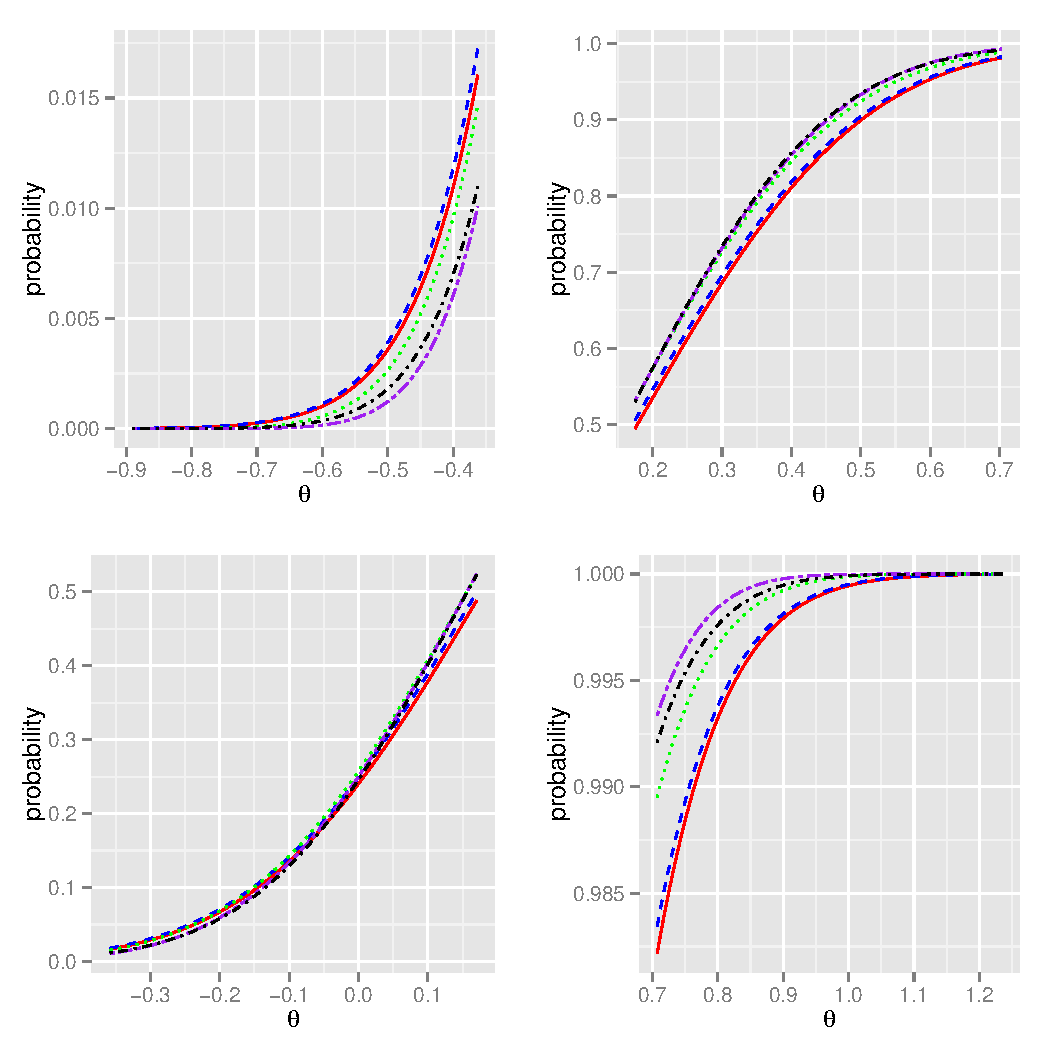
\includegraphics[scale=0.5]{n10bw.pdf}\protect\caption{Posterior cumulative distribution function when sample size is 10\label{fig:Posterior-CDF-n10}}
\end{center}

\end{figure}
\begin{figure}[H]

\begin{center}
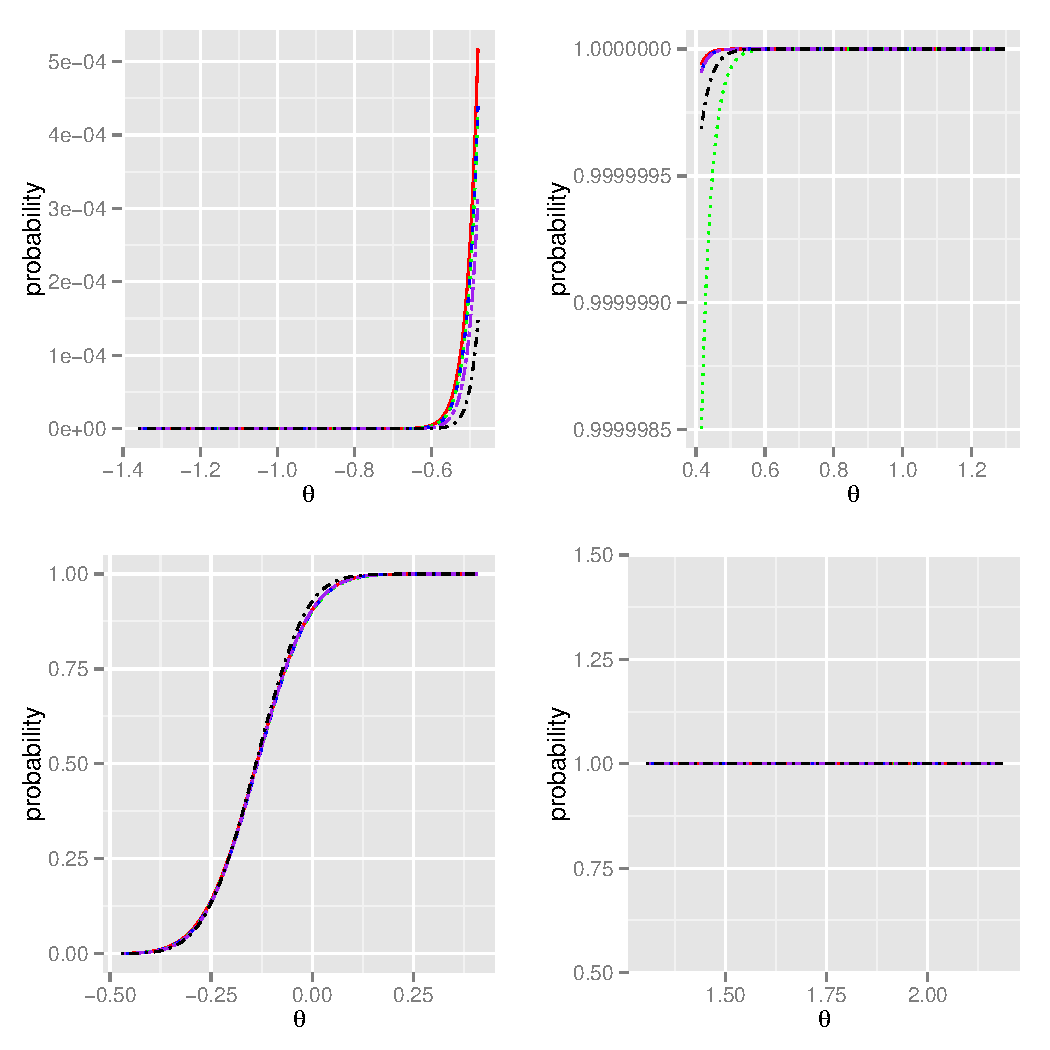
\includegraphics[scale=0.5]{n80bw.pdf}\protect\caption{Posterior cumulative distribution function when sample size is 80\label{fig:Posterior-CDF-n80}}
\end{center}

\end{figure}
 
\section{Discussion}
The paper provides an asymptotic expansion of the posterior based on an empirical likelihood subject to a linear constraint. The Bernstein --von Mises theorem and asymptotic expansions of the cumulative distribution function and the posterior mean are obtained as corollaries. Future work will include an extension to the multivariate case as well as expansions subject to multiple constraints. Another potential topic of research is asymptotic expansion of posteriors under regression constraints, extending the arguments of \cite{ghosal1999asymptotic,ghosal2000asymptotic}

